\documentclass[14pt,a4paper]{article}
\usepackage{ucs}
\usepackage{fancyhdr}
\usepackage{listings}
\usepackage{amsfonts}
\usepackage{amsmath}
\usepackage{setspace}
\usepackage{graphicx}
\usepackage{amssymb}
\usepackage{array}
\usepackage{subfigure}
\usepackage{listing}

\pagestyle{fancy}
\renewcommand\thesubsubsection{}
\renewcommand\thesubsection{\alph{subsection})}
\renewcommand\thesection{Exercise \arabic{section}}
\lhead{Exercise 2}
\rhead{Group 4}
\title{\textbf{Sheet 2} \\  \textbf{Motion Models and Robot Odometry}}
\author{Group 4 \\Urs Borrmann, Caner Hazirbas, FangYi Zhi}

\begin{document}
\maketitle
\onehalfspacing

\section{}
	\refstepcounter{subsection}
	\refstepcounter{subsection}
	\subsection{Group Picture}


	\subsection{Graph Visualization}


	\subsection{Specify the odometry model}


\section{}
	\refstepcounter{subsection}
	\refstepcounter{subsection}
	\refstepcounter{subsection}		
	\subsection{Kalman Filter Covariance Ellipse Screenshot}
		Figure \ref{graph:Q_origin} is the screenshot of the covariance ellipse from the original Q matrix visualized by rviz.\footnote{In order to easily compare the difference between the effect of the two diffenrent Q matrices, we took both screenshots at the last moment of the given bagfile.}\\
	
	\begin{figure}[htbp]
	\centering
	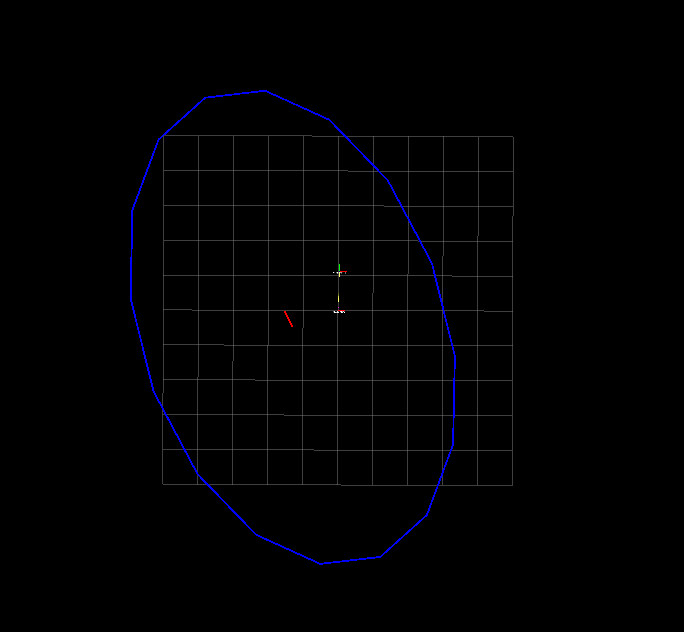
\includegraphics[scale=0.5]{Q_origin.png}
  	\caption{Covariance ellipse with the origin Q matrix}
    \label{graph:Q_origin}
	\end{figure}
	
	Figure \ref{graph:filtered_pose} shows the screenshot of the estimated two-dimensional trajectory from the given bag file.
	
	\begin{figure}[htbp]
	\centering
	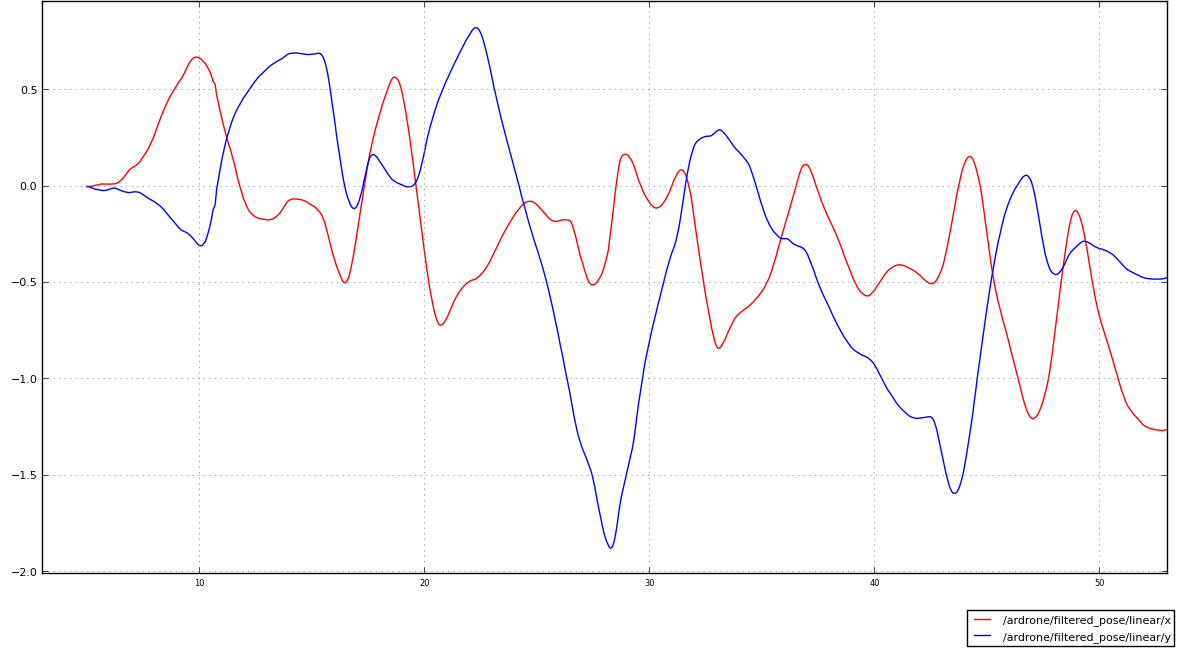
\includegraphics[scale=0.4]{filtered_pose.png}
  	\caption{Estimated two-dimensional trajectory from the given bag file}
    \label{graph:filtered_pose}
	\end{figure}
	

	\subsection{Kalman Filter with Higher Noise Screenshots}
	Figure \ref{graph:Q_2Times} shows the screenshot of the covariance ellipse from the modified Q matrix, which drifts two times more in the global x-direction.\\
	
	\begin{figure}[htbp]
	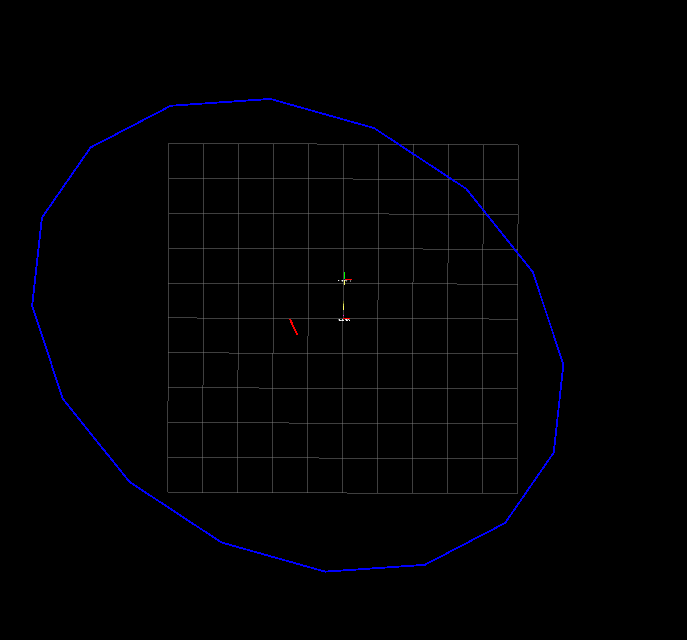
\includegraphics[scale=0.5]{Q_x_2Times.png}
  	\caption{Covariance ellipse with the modified Q matrix}
    \label{graph:Q_2Times}
	\end{figure}
	
		Figure \ref{graph:filtered_pose_modifiedQ} shows the screenshot of the estimated two-dimensional trajectory from the bag file with modified Q matrix.\footnote{There is no difference of the trajectories between the two different Q matrix, since until now, the Q matrix just adjusts the covariance ellipse but not the state vector, hence the trajectory.}
	
	\begin{figure}[htbp]
	\centering
	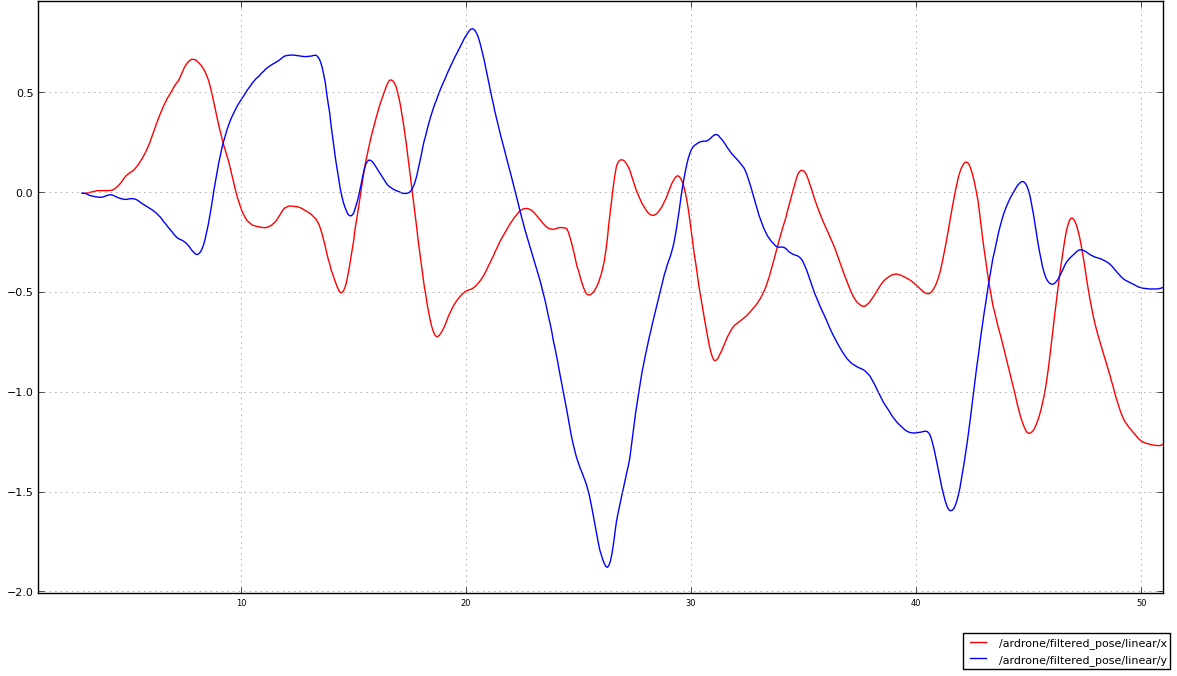
\includegraphics[scale=0.4]{filtered_pose_modifiedQ.png}
  	\caption{Estimated two-dimensional trajectory from the bag file with modified Q matrix.}
    \label{graph:filtered_pose_modifiedQ}
	\end{figure}
	
	\subsection{Noise Prediction for Experimental Setup}	
	
	\subsection{Observation Function and Its Jacobian}
		\subsubsection{Observation Function}
	 	Observed marker pose is calculated with function $h(x)$ (eq. 1). This $h(x)$ observation function predicts the marker pose $z_{pre}$ given $x$, estimated robot world state(eq 2), and $z_{g}$ ,the marker pose in global frame(eq. 3).
		 
		\begin{enumerate}
		\item $\begin{aligned}[t]
		    &&&&&&&&&&&&& \overrightarrow{z_{pre}} =h(\vec{x}) \\
		    &&&&&&&&&&&&& \overrightarrow{z_{pre}}  = (x_{pre}&&y_{pre}&\psi_{pre})^T
		\end{aligned}$
		\item $\begin{aligned}[t]
		    &&&&&&&&&&&&& \vec{x} = (x_{w}&&y_{w}&\psi_{w})^T
		\end{aligned}$
		\item $\begin{aligned}[t]
		    &&&&&&&&&&&&& \vec{z_{g}}  = (x_{g}&&y_{g}&\psi_{g})^T
		\end{aligned}$
		\end{enumerate}
	
		In order to find the observation, we need to transform the global marker pose to local frame.
		
		If X is homogeneous transformation matrix of $x$, robot pose,
		
		$$	X =	\begin{pmatrix} 
					R & t \\
					0 & 1 
				\end{pmatrix}
			=	\begin{pmatrix}
					\cos\psi_{w}	 &	-\sin\psi_{w} & x_{w}\\	
					\sin\psi_{w} &	\cos\psi_{w}	 & y_{w}\\
					0		 &		0	&	1
				\end{pmatrix}
		$$	
		
		then we can transform any local frame to global frame as follows;
		
				\[\vec{t_g}= X \overrightarrow{t_{pre}} \]
				
		We want to transform from global to local. In order to do that we should take inverse of X transformation matrix;
		$$	X^{-1} =	\begin{pmatrix} 
		
					R^{-1} & -R^{-1}t \\
					0 & 1 
				\end{pmatrix}
			=	\begin{pmatrix}
					\cos\psi_{w}	 &	\sin\psi_{w} & -x_{w}\cos\psi_{w}-y_{w}\sin\psi_{w}\\	
					-\sin\psi_{w} &	\cos\psi_{w}	 &  x_{w}\sin\psi_{w}-y_{w}\cos\psi_{w}\\
					0		 &		0	&	1
				\end{pmatrix}
		$$
		
		
		Now we can compute the local marker position from global marker position;
		
		\[\vec{t_{g}}= \left( \begin{array}{c}
						x_{g} \\ y_{g}\\ 1\\
				\end{array} \right)\] 	
		$$
			\tilde{t_{pre}}  = X^{-1} \tilde{t_{g}}
			= \begin{pmatrix}
					(x_{g} - x_{w})\cos\psi_{w}	 +	(y_{g}-y_{w})\sin\psi_{w}\\ 	
					-(x_{g} - x_{w})\sin\psi_{w} +	(y_{g}-y_{w})\cos\psi_{w}\\
												1
				\end{pmatrix}
		$$
		
		Since yaw angle is always in the global frame, predicted yaw angle is
		
		\[ \psi_{pre}=(\psi_{g} - \psi_{w})\]
		
		At the end we get the following observation function
		
		$$
		h(\vec{x})	= \begin{pmatrix}
					(x_{g} - x_{w})\cos\psi_{w}	 +	(y_{g}-y_{w})\sin\psi_{w}\\ 	
					-(x_{g} - x_{w})\sin\psi_{w} +	(y_{g}-y_{w})\cos\psi_{w}\\
											(\psi_{g} - \psi_{w})
			\end{pmatrix}
		$$
		
		Its derivative (Jacobian) can be then calculated as:
				$$
		H(\vec{x})	= \frac{\partial h(\vec{x})}{\partial \vec{x}} = 
			\begin{pmatrix}
				-\cos\psi_{w} & -\sin\psi_{w} & -(x_g-x_w)\sin\psi_{w}+(y_g-y_w)\cos\psi_{w} \\
				\sin\psi_{w} & -\cos\psi_{w} & -(x_g-x_w)\cos\psi_{w}-(y_g-y_w)\sin\psi_{w} \\
				0 & 0 & -1 
			\end{pmatrix}
		$$
		
		
	\refstepcounter{subsection}
	\subsection{Trajectory}
		Figure \ref{graph:filtered_pose_corrected} shows the screenshot of the from EKF corrected two-dimensional trajectory from the given bag file.
	
	\begin{figure}[htbp]
	\centering
	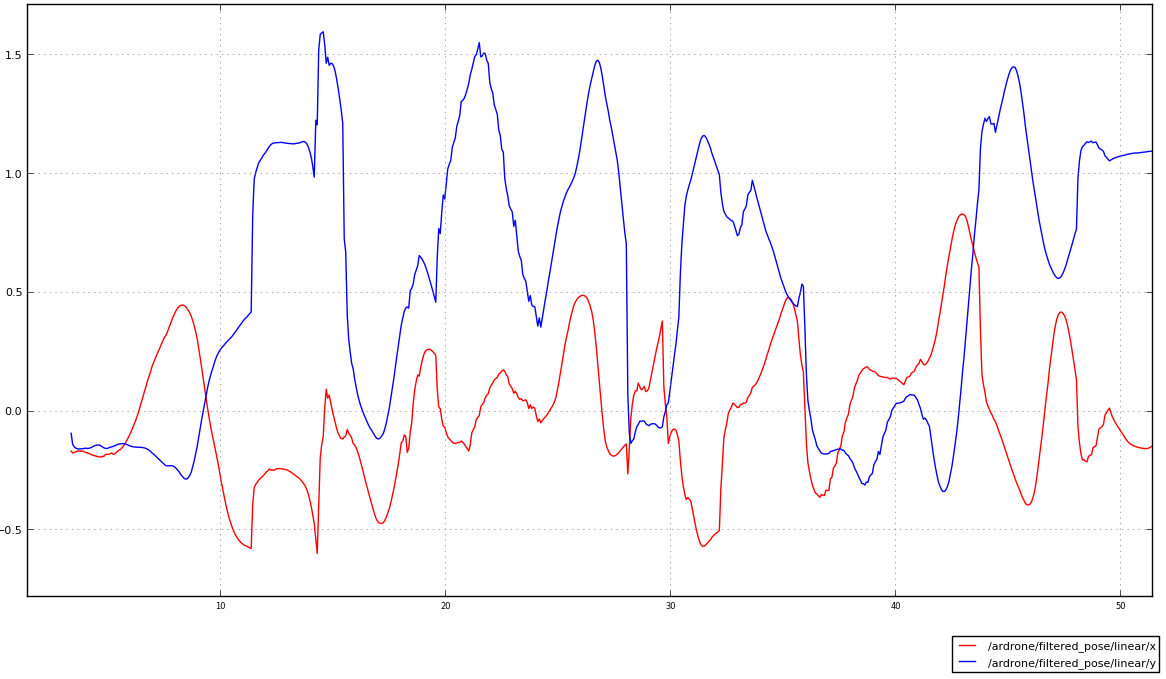
\includegraphics[scale=0.4]{filtered_pose_corrected.png}
  	\caption{From the EKF corrected two-dimensional trajectory from the given bag file}
    \label{graph:filtered_pose_corrected}
	\end{figure}
		
	
	\subsection{Drift on Pose Estimation}
	

\end{document}
